\subsubsection{Moduł autentykacji}
Struktura:
\begin{itemize}
	\item storage/src/auth/storage\_auth\_srv.erl – gen\_server
	\item storage/src/auth/db\_users.erl – DAO dla struktur User
\end{itemize}

Moduł autentykacji odpowiada za obliczanie i weryfikację sumy kontrolnej HMAC przekazywanych zapytań. Moduł db\_users jest modułem dostępowym do encji reprezentujących użytkownika (struktury User), przechowywanych w bazie danych. Suma HMAC opisana jest dokładniej w kolejnym punkcie.

\begin{figure}[!htbp]
	\centering
	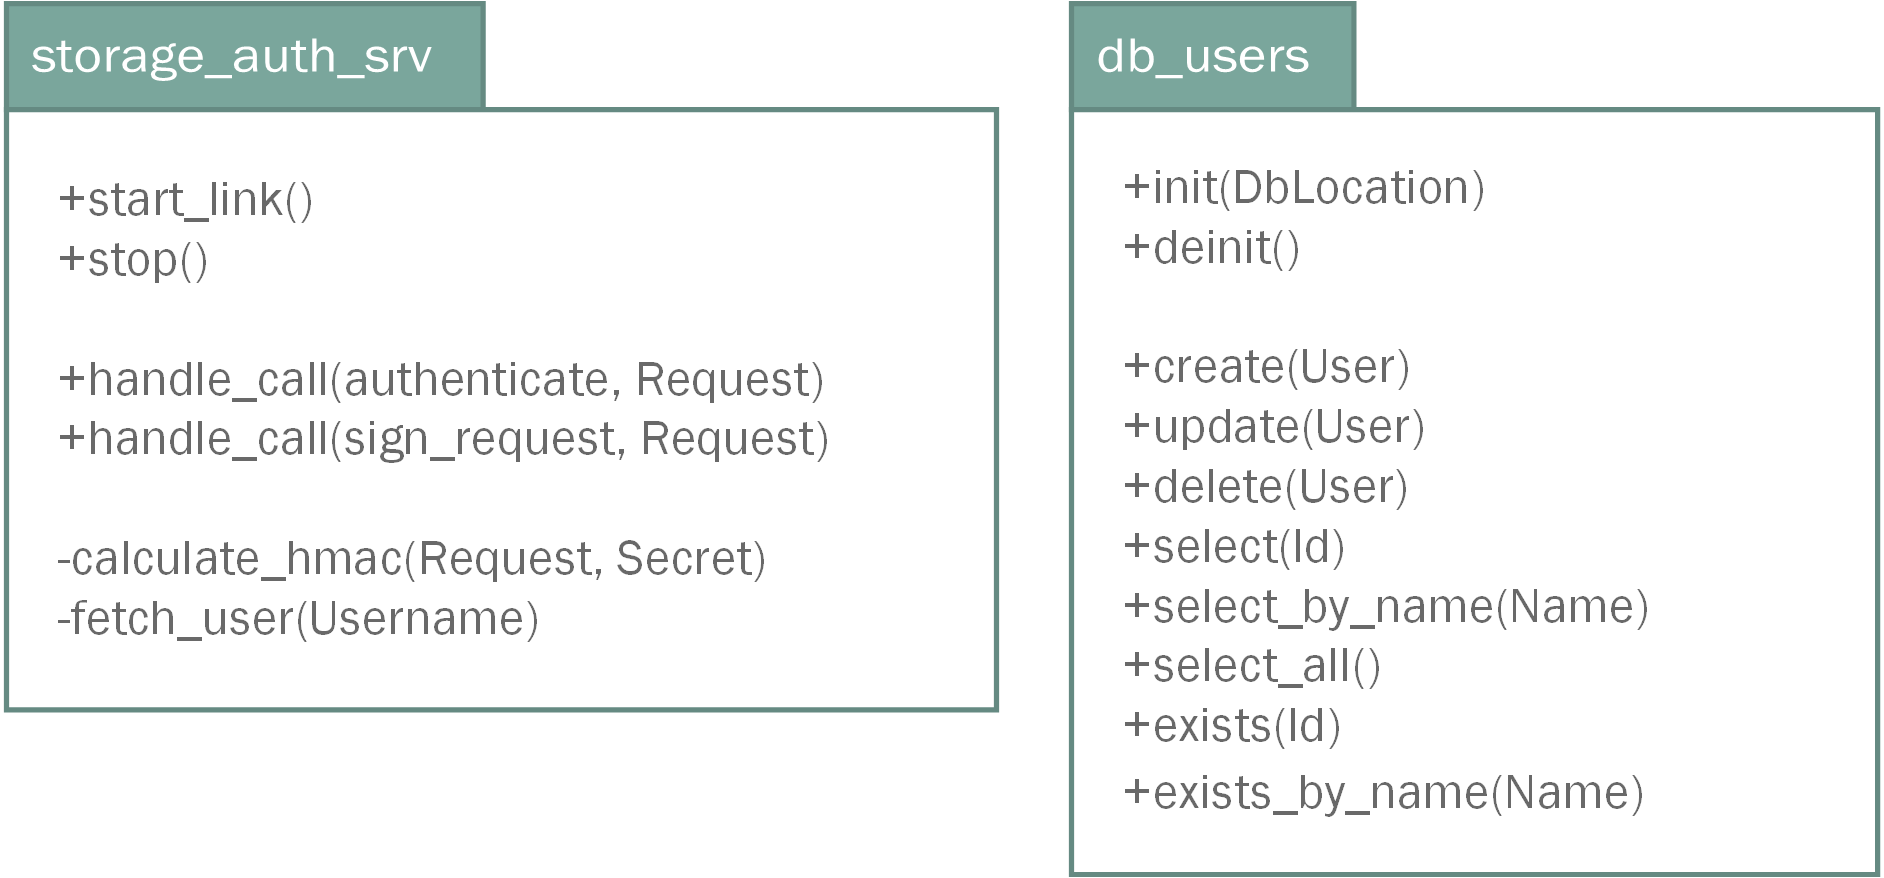
\includegraphics[width=0.9\textwidth]{auth-module}
	\caption[Budowa modułu autentykacji.]{Moduły składające się na moduł autentykacji. storage\_auth\_srv pozwala na porównanie sumy kontrolnej otrzymanego zapytania z wartością, którą sam wylicza. db\_users oferuje podstawowe operacje na bazie użytkowników, z wykorzystaniem struktury User.}
	\label{fig:auth-module}
\end{figure}

Serwer storage\_auth\_srv przechowuje tablicę ets zawierającą krotki {Username, Secret, Expires}, pełniącą rolę pamięci podręcznej. Znajdują się w niej użytkownicy wraz z ich kluczami prywatnymi. Opis aktualizacji tej tablicy znajduje się w rozdziale Synchronizacja użytkowników.

\paragraph{Suma HMAC:} keyed-Hash Message Authentication Code to funkcja skrótu z dodatkowo wmieszanym kluczem prywatnym. Wynikowy kod zależy nie tylko od danych z których jest obliczany, ale również od wykorzystanego hasła. Hasło (klucz prywatny) znane jest tylko użytkownikowi oraz systemowi. Nie jest przesyłane między nimi, co zmniejsza szanse na ujawnienie klucza.

Wykorzystanie HMAC zapewnia ochronę integralności przesyłanych zapytań (modyfikacja parametrów zapytania wymaga przeliczenia sumy HMAC) oraz autentyczności danych (wyliczenie sumy wymaga znajomości klucza prywatnego).

Każdy użytkownik posiada "hasło". Może on je ustalić dowolnie ze swoimi preferencjami. Kluczem prywatnym staje się suma SHA1 obliczona z tego hasła, i tylko ta wartość przechowywana jest w bazie danych.
